\documentclass[aspectratio=169,11pt]{beamer}
\usetheme{Madrid}
\usecolortheme{seahorse}
\usepackage[T1]{fontenc}
\usepackage{lmodern}
\usepackage{booktabs,graphicx,amsmath,tikz,xcolor,array}
\usetikzlibrary{shapes,arrows.meta,positioning}
\definecolor{good}{RGB}{30,130,76}
\definecolor{bad}{RGB}{192,57,43}
\setbeamertemplate{navigation symbols}{}
\title[AnomalyGFM: Anomaly2]{Beyond the Single Prototype: MoE, Test-Time Adaptation, Edge Purification and PPR Residuals for AnomalyGFM}
\subtitle{Second study --- what works, what breaks, and why}
\author{Term project team}
\date{\today}

\begin{document}
\begin{frame}\titlepage\end{frame}
\begin{frame}{Outline}\tableofcontents\end{frame}

\section{Context}
\begin{frame}{AnomalyGFM in one slide}
\begin{columns}[T]
\column{0.52\textwidth}
\begin{itemize}\small
\item Pre-train \emph{once} on one graph (Facebook), detect anomalies in unseen graphs \alert{zero-shot}.
\item Node \textbf{residual} $r_v=h_v-\sum_{u}P_{vu}h_u$ (1-hop neighbour mean): small for normal, large for anomalous nodes.
\item \textbf{One} learnable abnormal prototype $p_a$; score $s_v=\exp\cos(r_v,p_a)$.
\item Adjacency is \alert{trusted blindly}; no adaptation to the target without labels.
\end{itemize}
\column{0.48\textwidth}
\includegraphics[width=\linewidth]{../../framework.png}
\end{columns}
\end{frame}

\begin{frame}{Four weaknesses $\rightarrow$ four extensions}
\centering
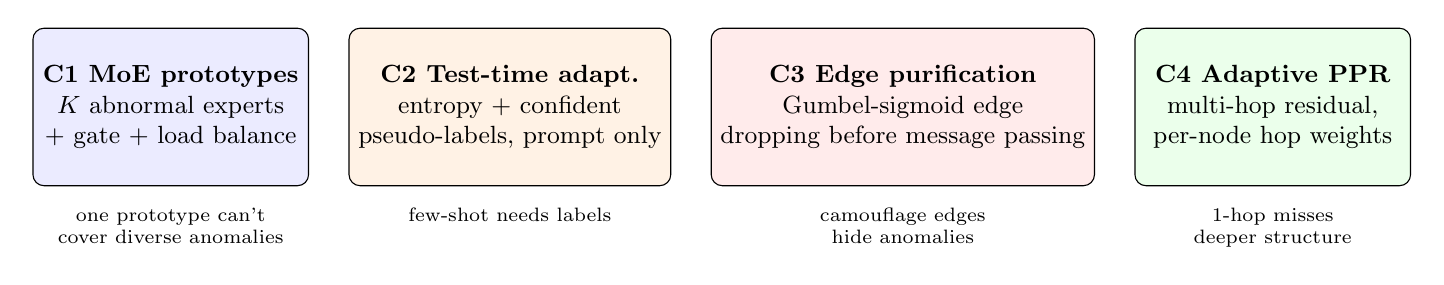
\begin{tikzpicture}[box/.style={draw,rounded corners,align=center,minimum width=3.5cm,minimum height=2.0cm,font=\small},>=Stealth]
\node[box,fill=blue!8] (a) {\textbf{C1 MoE prototypes}\\$K$ abnormal experts\\+ gate + load balance};
\node[box,fill=orange!10,right=0.5cm of a] (b) {\textbf{C2 Test-time adapt.}\\entropy + confident\\pseudo-labels, prompt only};
\node[box,fill=red!8,right=0.5cm of b] (c) {\textbf{C3 Edge purification}\\Gumbel-sigmoid edge\\dropping before message passing};
\node[box,fill=green!8,right=0.5cm of c] (d) {\textbf{C4 Adaptive PPR}\\multi-hop residual,\\per-node hop weights};
\node[below=0.15cm of a,font=\scriptsize,text width=3.4cm,align=center]{one prototype can't cover diverse anomalies};
\node[below=0.15cm of b,font=\scriptsize,text width=3.4cm,align=center]{few-shot needs labels};
\node[below=0.15cm of c,font=\scriptsize,text width=3.4cm,align=center]{camouflage edges hide anomalies};
\node[below=0.15cm of d,font=\scriptsize,text width=3.4cm,align=center]{1-hop misses deeper structure};
\end{tikzpicture}
\end{frame}

\begin{frame}{Protocol (real graphs only)}
\begin{columns}[T]
\column{0.55\textwidth}
\begin{itemize}\small
\item \textbf{Train:} Facebook (1,081 nodes; 30\% labelled; 301 epochs; the paper's recipe)
\item \textbf{Zero-shot targets:} Amazon (11,944), Amazon-UPU (10,224), Reddit (10,984), Elliptic (46,564)
\item \textbf{5 seeds}, AUROC/AUPRC on all target nodes; params; peak GPU memory
\item \textbf{Controls} isolate each idea (attack-augmentation without purifier; TTA with shuffled pseudo-labels)
\item Attack benchmark perturbs only the \emph{edge set} of real graphs
\end{itemize}
\column{0.45\textwidth}
\begin{block}{Infrastructure}\small RTX 4500 Ada (24 GB); code local, jobs run on the server (\texttt{sync.sh}); sparse GPU operators.\\
Baseline reproduces the first study exactly (seed 0 Amazon AUROC 0.8603).\end{block}
\end{columns}
\end{frame}

\section{Headline}
\begin{frame}{Headline: no extension improves average AUROC}
\centering\scriptsize
\begin{tabular}{lccccccc}
\toprule
Method & Amazon & UPU & Reddit & Elliptic & \textbf{Avg AUROC} & Avg AUPRC & GPU MB\\ \midrule
Baseline AnomalyGFM & .834 & .792 & .573 & .394 & \textbf{.648} & .244 & 626\\
+ C1 MoE (K=4) & .820 & .793 & .556 & .399 & .642 & .226 & 630\\
+ C2 TTA (30 steps) & .812 & .796 & .551 & .418 & .644 & .211 & 860\\
\hspace{3pt}ctrl: shuffled pseudo-labels & .840 & .795 & .556 & .417 & .652 & .247 & 860\\
+ C3 Edge purification & .824 & .758 & .500 & \textcolor{good}{\textbf{.499}} & .645 & .252 & 1,675\\
\hspace{3pt}ctrl: attack-aug, no purifier & .799 & .771 & .528 & .372 & .617 & .213 & 640\\
+ C4 Adaptive PPR & .834 & .795 & .558 & .395 & .646 & .251 & 675\\
C1+C3+C4 combined & .825 & .753 & .482 & .499 & .640 & .220 & 1,706\\ \bottomrule
\end{tabular}
\vspace{6pt}
\begin{itemize}\footnotesize
\item Differences of the average are within seed noise ($\sigma=0.009$--$0.037$). Params: +3,204 (C1), +80 updated (C2), +705 (C3), +132 (C4).
\item What \emph{is} robust is narrower: C3 under attack, C4's learned hop gate, and why C1/C2 fail (next slides).
\end{itemize}
\end{frame}

\section{C1: MoE}
\begin{frame}{C1: Mixture-of-Experts abnormal prototypes}
\begin{columns}[T]
\column{0.52\textwidth}
\textbf{Experts:} $p_k=\mathrm{ReLU}(W_{abn}\epsilon_k+\delta_k)$, $k\le K$\\
\textbf{Gate:} $g_v=\mathrm{softmax}\big(\mathrm{Linear}(r_v/\|r_v\|)\big)$\\
\textbf{Score:} $s_v=\sum_k g_{vk}\cos(r_v,p_k)$
\[
\mathcal L=\sum_k g_{vk}\|p_k-r_v\|+\lambda_{lb}K\!\sum_k f_kP_k+\lambda_{div}\,\overline{\cos(p_k,p_l)}
\]
\footnotesize load balancing (Switch-style) + expert diversity; +3,204 params.
\column{0.48\textwidth}
\footnotesize
\begin{tabular}{rcccc}
\toprule
K & Amazon & UPU & Reddit & Ellip.\\ \midrule
1 (paper) & \textbf{.834} & .792 & \textbf{.573} & .394\\
2 & .827 & .796 & .563 & .405\\
4 & .820 & .793 & .556 & .399\\
8 & .812 & .791 & .547 & .406\\ \bottomrule
\end{tabular}\\[5pt]
AUROC; $\lambda$'s and lr chosen on Facebook only.
\begin{itemize}\footnotesize
\item AUROC \emph{decreases} slowly with $K$ on Amazon/Reddit; flat elsewhere.
\end{itemize}
\end{columns}
\end{frame}

\begin{frame}{C1: routing collapses --- t-SNE of residuals (Amazon)}
\begin{columns}[T]
\column{0.68\textwidth}
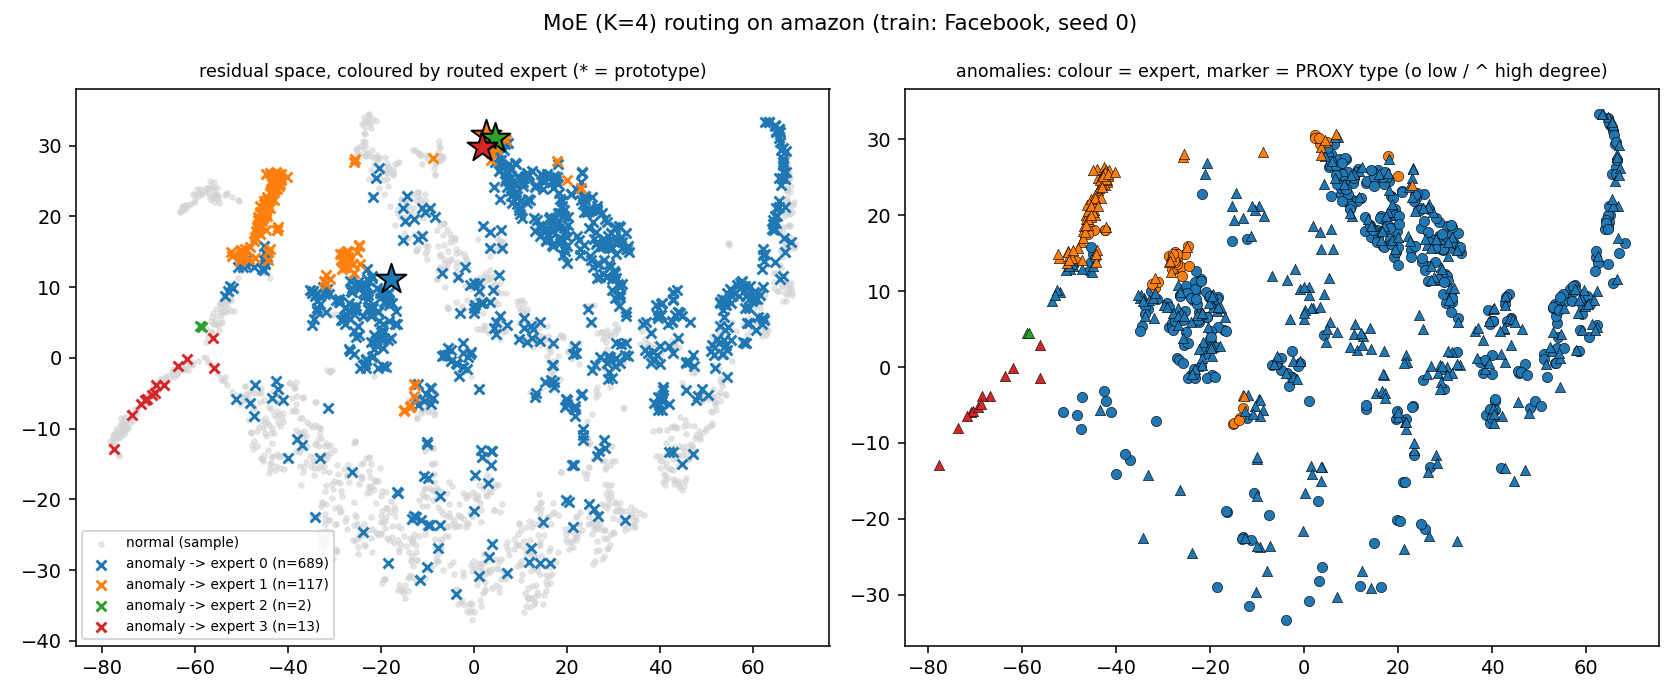
\includegraphics[width=\linewidth]{../results/moe_tsne_amazon.png}
\column{0.32\textwidth}
\footnotesize
\textbf{Expert usage} (821 anomalies):\\ Amazon [689, 117, 2, 13]\\ UPU [438, 220, 7, 28]\\ Reddit [366, 0, 0, 0]\\[4pt]
Silhouette 0.145 / 0.076.\\[4pt]
\textcolor{good}{Experts 1 \& 3 occupy separate regions.}\\
\textcolor{bad}{Expert 0 takes 84\% (Reddit: 100\%).}\\[4pt]
\alert{No dataset has anomaly-type labels} $\Rightarrow$ we cannot claim experts = types; assignment correlates with a degree \emph{proxy} ($p<10^{-4}$). Only $\approx$7 labelled anomalies in the training split.
\end{columns}
\end{frame}

\section{C2: TTA}
\begin{frame}{C2: unsupervised test-time adaptation}
\begin{columns}[T]
\column{0.55\textwidth}
\textbf{Update only an 80-parameter input prompt} on the unlabeled target:
\begin{enumerate}\footnotesize
\item score $\to$ robust $z$ $\to$ $p_v=\sigma\big((z_v-q)/T\big)$, $q$ = assumed 5\% contamination quantile
\item pseudo-labels: $p>0.95$ anomaly, $p<0.05$ normal
\item loss $=$ BCE(confident) $+\,0.1\cdot$entropy(all)
\end{enumerate}
\footnotesize Ground truth used \emph{only} to log AUROC/AUPRC per step. Control: shuffled pseudo-labels.
\column{0.45\textwidth}
\footnotesize
\begin{tabular}{lcccc}
\toprule
$\Delta$AUROC & Amz & UPU & Red & Ell\\ \midrule
lr $10^{-3}$ & \textcolor{bad}{$-.028$} & $+.005$ & \textcolor{bad}{$-.030$} & $+.042$\\
lr $10^{-2}$ & \textcolor{bad}{$-.113$} & $-.016$ & \textcolor{bad}{$-.085$} & $+.140$\\
shuffled ctrl & $-.338$ & $-.230$ & $-.055$ & \textcolor{bad}{$+.127$}\\
pseudo-pos. prec. & .75 & .65 & .007 & .002\\
base rate & .069 & .068 & .033 & .098\\ \bottomrule
\end{tabular}
\end{columns}
\end{frame}

\begin{frame}{C2: learning curves (no labels used for adaptation)}
\begin{columns}[T]
\column{0.5\textwidth}
\centering\footnotesize\textbf{Amazon} --- pseudo-labels good (75\%)\\
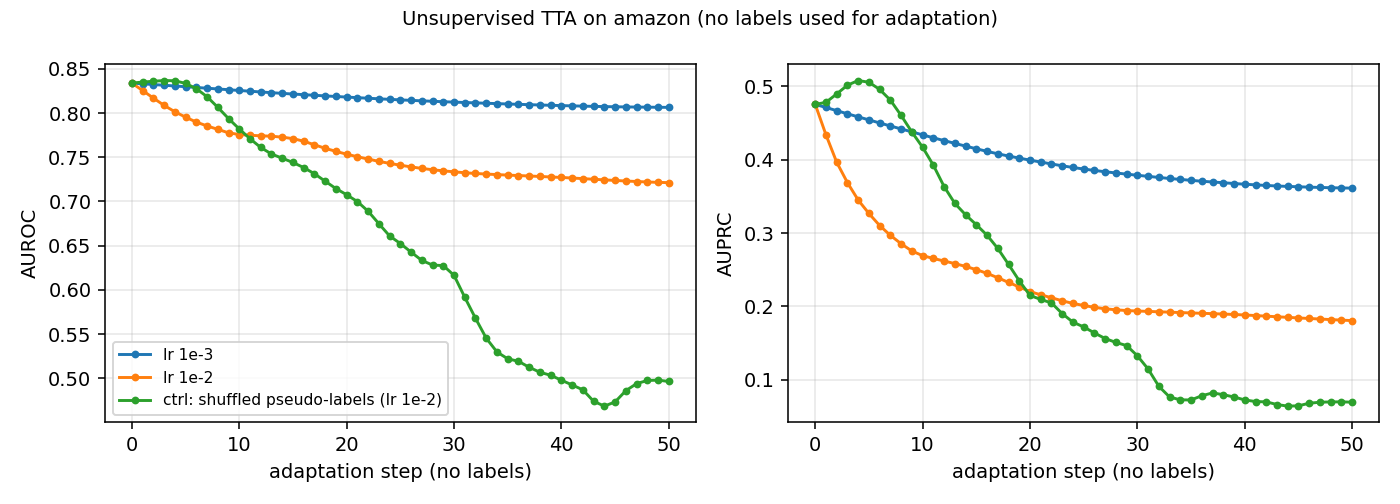
\includegraphics[width=\linewidth]{../results/tta_curves_amazon.png}
\column{0.5\textwidth}
\centering\footnotesize\textbf{Elliptic} --- pseudo-labels worse than chance\\
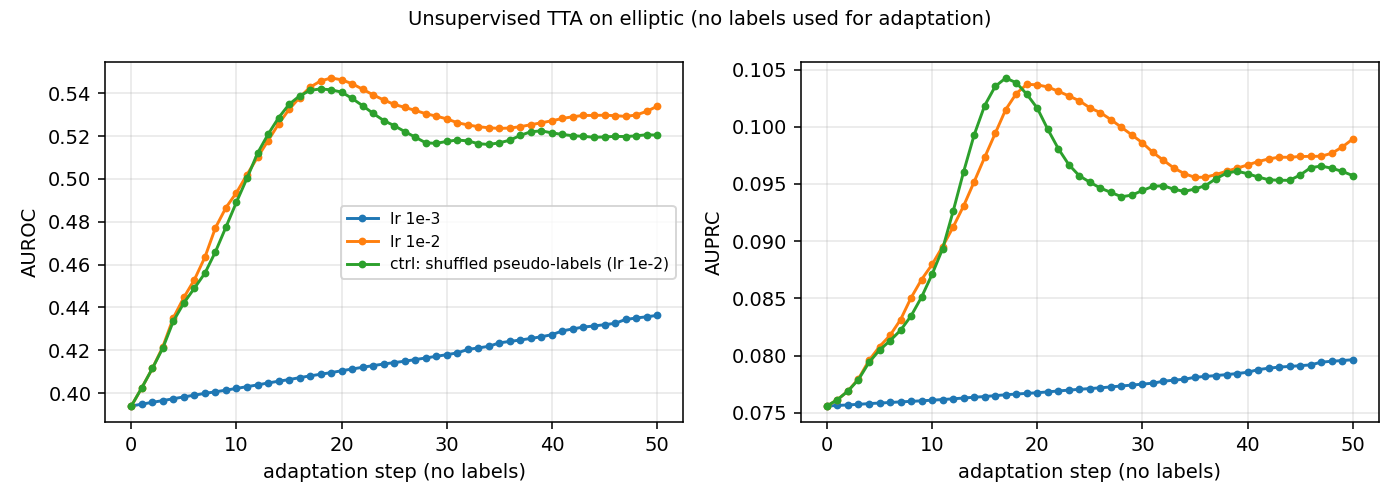
\includegraphics[width=\linewidth]{../results/tta_curves_elliptic.png}
\end{columns}
\vspace{2pt}
\begin{itemize}\footnotesize
\item Good pseudo-labels \emph{still} hurt (entropy sharpening). Elliptic's gain is matched by \textbf{random} pseudo-labels $\Rightarrow$ not label-free learning.
\end{itemize}
\end{frame}

\section{C3: Edge purification}
\begin{frame}{C3: adversarial edge purification}
\begin{columns}[T]
\column{0.52\textwidth}
\textbf{Scorer} (symmetric edge features $\Rightarrow w_{uv}=w_{vu}$): $|x_u-x_v|$, $x_u\!\odot\! x_v$, degrees, \alert{common neighbours + Salton overlap} $\to$ MLP.\\[3pt]
\textbf{Train:} Gumbel-sigmoid $w=\sigma\big((\ell+\eta)/\tau\big)$; \textbf{test:} hard drop $\ell\le0$.\\[3pt]
\textbf{Adversarial training:} each epoch (50\%) inject 10\% random + 10 camouflage edges per anomaly; injected edges are known $\Rightarrow$ edge-level BCE.\\[3pt]
\footnotesize Weights re-weight both the GCN operator and the neighbour mean (before the residual); 705 params.
\column{0.48\textwidth}
\small\textbf{Design history (source graph only)}\\[2pt]
\footnotesize
\begin{tabular}{lcc}
\toprule
 & edge-AUROC & real edges dropped\\ \midrule
paper lr $10^{-4}$ & \textcolor{bad}{0.30} & 0\% (no-op)\\
node features only & 0.70 & \textcolor{bad}{48\%}\\
+ common neighbours & \textcolor{good}{\textbf{0.96}} & \textcolor{good}{3--4\%}\\ \bottomrule
\end{tabular}\\[5pt]
\scriptsize Held-out Facebook AUROC, clean / attacked:\\ purified 0.839 / 0.735 vs no purifier 0.741 / 0.610.
\end{columns}
\end{frame}

\begin{frame}{C3: the baseline crashes under camouflage --- the purifier holds}
\centering\small\textbf{Amazon-UPU, AUROC (5 seeds)}\\[3pt]
\footnotesize
\begin{tabular}{lcccccc}
\toprule
 & clean & camo 5 & camo 20 & camo 50 & rewire 30\% & rewire 50\%\\ \midrule
Baseline & .792 & .669 & .244 & \textcolor{bad}{\textbf{.085}} & \textbf{.822} & \textbf{.819}\\
Baseline + attack-aug (ctrl) & .771 & .632 & .164 & .046 & .799 & .793\\
\textbf{Edge-purified} & .760 & \textbf{.734} & \textbf{.701} & \textcolor{good}{\textbf{.678}} & .667 & .617\\ \bottomrule
\end{tabular}
\vspace{5pt}
\begin{itemize}\footnotesize
\item Camouflage ($m$ random normal neighbours per anomaly) \alert{inverts the baseline's ranking}; edge-level diagnostic: purifier AUROC \textbf{0.99}, drops 99.5\% of injected vs 4.7\% of real edges.
\item \textcolor{bad}{But:} worse than baseline under random rewiring (it deletes real edges too); Amazon (avg degree 736) is barely affected by either attack.
\end{itemize}
\end{frame}

\begin{frame}{C3: where it fails --- and where it helps}
\begin{columns}[T]
\column{0.5\textwidth}
\textcolor{bad}{\textbf{Reddit: fails}}
\begin{itemize}\footnotesize
\item Reddit has \textbf{zero common neighbours} on every edge (triangle-free).
\item Facebook-learned ``no shared neighbours $=$ fake'' deletes 96\% of real edges; clean AUROC 0.50.
\item Under camouflage 50: 0.300 vs baseline 0.029 --- still $<0.5$.
\end{itemize}
\column{0.5\textwidth}
\textcolor{good}{\textbf{Elliptic: helps}}
\begin{itemize}\footnotesize
\item AUROC \textbf{0.499} vs baseline 0.394 and control 0.372 ($+0.105$, $+0.127$).
\item Still only chance level --- it removes an \emph{inversion}, not a solution.
\end{itemize}
\textbf{Cost:} peak GPU 1.7 GB vs 0.6 GB (common-neighbour computation).
\end{columns}
\end{frame}

\section{C4: PPR}
\begin{frame}{C4: adaptive multi-hop (PPR) residual}
\begin{columns}[T]
\column{0.5\textwidth}
\[
r_v=h_v-\sum_{k=1}^{K}w_{vk}\,(P^{k}h)_v
\]
\small
\begin{itemize}
\item \texttt{hop1}: paper \quad \texttt{hop2}: 0.5/0.5
\item \texttt{ppr}: $w_k\propto(1-\alpha)^{k-1}$, $\alpha=0.3$
\item \texttt{adaptive}: $w_v=\mathrm{softmax}\big(\log\text{prior}+\mathrm{MLP}(\text{structure}_v)\big)$, zero-init $\Rightarrow$ starts at PPR
\end{itemize}
\footnotesize $K{=}4$ sparse mat-muls, no $N\!\times\!N$ matrix; +132 params.
\column{0.5\textwidth}
\footnotesize
\begin{tabular}{lcccccc}
\toprule
AUROC & Amz & UPU & Red & Ell & Tol & \textbf{Avg}\\ \midrule
1-hop (paper) & .834 & .792 & .573 & .394 & .538 & \textbf{.626}\\
2-hop & .819 & .792 & .531 & .380 & .544 & .613\\
PPR & .815 & .790 & .534 & .372 & .540 & .610\\
\textbf{Adaptive} & .834 & .795 & .558 & .395 & .532 & .623\\ \bottomrule
\end{tabular}\\[4pt]
AUPRC avg: .249 / .233 / .225 / \textbf{.254}
\end{columns}
\end{frame}

\begin{frame}{C4: the gate learns an adaptive receptive field --- but it only ties 1-hop}
\centering\small
\begin{tabular}{lcccc}
\toprule
Mean learned hop weights & hop 1 & hop 2 & hop 3 & hop 4\\ \midrule
PPR prior ($\alpha=0.3$) & .395 & .276 & .193 & .135\\
Facebook (train) & .785 & .003 & .003 & .210\\
Amazon & .801 & .006 & .005 & .188\\
Reddit & .788 & .006 & .006 & .200\\
Elliptic & .853 & .002 & .003 & .142\\ \bottomrule
\end{tabular}
\vspace{6pt}
\begin{itemize}\footnotesize
\item Within-graph std $\approx0.27$--$0.30$: \textbf{bimodal per node} --- most nodes compare with their 1-hop mean, a minority with a 4-hop reference; same pattern on every graph.
\item Fixed multi-hop references are \textcolor{bad}{worse} (dilute the contrast). Adaptive \emph{recovers} 1-hop accuracy but does not beat it --- \alert{not even on Elliptic} (laundering structures): 0.395 vs 0.394.
\item $P^k$ is a walk operator: even hops include returns to the node.
\end{itemize}
\end{frame}

\section{Process}
\begin{frame}{A process lesson: round 1 vs round 2}
\begin{columns}[T]
\column{0.55\textwidth}
\textbf{Round 1} (new modules trained at the paper's lr $10^{-4}$): everything collapsed. Diagnostics showed:
\begin{itemize}\footnotesize
\item purifier \textbf{dropped 0\% of edges}; edge-AUROC 0.30 \emph{on the training graph}
\item adaptive gate $\equiv$ fixed PPR (never moved)
\item controls: the damage came from the augmentation, not the purifier
\end{itemize}
\textbf{Fix} (selected on Facebook only): per-module learning rates, common-neighbour edge features, un-balanced edge loss, augmentation strength.\\[3pt]
\scriptsize\alert{Honesty note:} I saw round-1 target results before redesigning the purifier; hyper-parameters came from the source only, but round 2 is not fully blind.
\column{0.45\textwidth}
\centering\small
\begin{tabular}{lcc}
\toprule
Avg AUROC & Round 1 & Round 2\\ \midrule
Baseline & .648 & .648\\
C1 MoE & .639 & .642\\
C3 purifier & \textcolor{bad}{.559} & \textcolor{good}{.645}\\
C4 adaptive & .626 & .646\\
combined & \textcolor{bad}{.494} & .640\\ \bottomrule
\end{tabular}
\end{columns}
\end{frame}

\section{Wrap-up}
\begin{frame}{What we can and cannot claim}
\begin{columns}[T]
\column{0.5\textwidth}
\textcolor{good}{\textbf{Can claim}}
\begin{itemize}\footnotesize
\item The paper's residual is \textbf{fragile to camouflage} (ranking inverts: 0.792$\to$0.085).
\item C3 with structural edge features detects injected edges (0.99) and keeps 0.68 under 50-edge camouflage; improves Elliptic over baseline \emph{and} control.
\item An adaptive PPR gate learns per-node hop choice.
\item MoE routing collapses with $\approx$7 labelled anomalies.
\item Self-training only works when the zero-shot ranking is already good.
\end{itemize}
\column{0.5\textwidth}
\textcolor{bad}{\textbf{Cannot claim}}
\begin{itemize}\footnotesize
\item Any average accuracy gain.
\item That MoE experts are anomaly \emph{types} (no type labels exist).
\item That C3 helps without triangles or under random noise.
\item Generality beyond 4 targets / one source graph.
\item A fully blind round 2.
\end{itemize}
\end{columns}
\end{frame}

\begin{frame}{Next steps and reproducibility}
\begin{columns}[T]
\column{0.5\textwidth}
\textbf{Next steps}
\begin{itemize}\small
\item Graph-agnostic purifier (per-graph normalised structure; learned embeddings) --- fixes Reddit
\item Multi-source pre-training for MoE (more labelled anomalies)
\item Consensus pseudo-labels + stopping rule for TTA
\item Non-backtracking walks for C4
\end{itemize}
\column{0.5\textwidth}
\textbf{Reproduce} (\texttt{Anomaly2/}):\\
\footnotesize\texttt{python main.py all}\\ (about 15 min, one RTX 4500 Ada)\\[4pt]
\texttt{README.md}: hooks into the official code\\ \texttt{WORK.md}: full story\\ \texttt{reports/C1--C4}: details\\[4pt]
\scriptsize github.com/SumitKumar-17/AnomalyGFM\\ (branch \texttt{team-contributions}, folder \texttt{Anomaly2/})
\end{columns}
\end{frame}
\end{document}
